\documentclass[../main.tex]{subfiles}	



\begin{document}

\chapter{Complex Analysis}
\label{ch:cmplx_analysis}

\section*{Introduction}

At present, the vast majority of deep learning architectures are based on real-valued operations and representations. However people knew that there was a numerical domain even larger, and more general, than the real one: the complex space $\mathds{C}$. We cannot forget also about the fact that Quantum Mechanics told us that the "true nature" of reality is inherently complex (since quantum states and operators lives in a complex Hilber space).\\ 
All of this is implicitly suggesting that actual deep learning techniques can be further extended to an even more general, and hopefully more efficient, representation. This possibility was already under the eyes of researchers from the dawn of deep learning, since the first publications covering this hypotheses are almost thirty years old.\\
In this chapter we are going to recall the main concepts, from complex analysis, that will be helpful during the practical extent of real-valued deep learning techniques in the complex world. We will address the main issues encountered in this development, mainly due to characteristics of the complex domain without an effective real counterpart (e.g. Liouville's and Identity theorems), but we will also focus on the property known as \textit{circularity}, that in principle could be the key to prove the effective advantages brought by complex-valued models. In the end, we will examine the core of modern deep learning approaches in presence of a complex dataset, focused on the existing mapping between numbers in $\mathds{C}$ and points in $\mathds{R}^2$, proving that in many cases it is inadequate, and should be replaced with a new and proper methodology living in the complex domain.

\section{Complex Numbers}
\label{sec:cmplx_numbers}

A natural way to build complex-valued neural networks is to extend real-valued models to handle complex-valued neurons. Obviously, this extension requires also the parameters (weights, biases) and the activations to be complex-valued. In contrast, the loss function should be real-valued, in order to allow for an empirical risk minimization during the training process. Despite all the operations that need to be redefined for this adaptation, the most challenging part of the problem consist into constructing a coherent and stable algorithm to train such networks.\\
The benefits of retaining a complex representation remains an open question; however, several works and implementations have recently proved that complex networks could leverage mathematical properties of $\mathds{C}$ to learn more efficient transform functions than with real-valued networks.\\
But, before getting into the motivation and background for complex-valued deep learning, we should first recall a few concepts of \textit{complex analysis} \footnote{A nice book to recall all the concepts explained is \cite{stein_complex_analysis}.}. 
\begin{definition}
A \textbf{complex number} $z\in\mathds{C}$ takes the form 
\[ z = x+iy \] 
where $x\in\mathds{R}$ and $y\in\mathds{R}$ are its real and imaginary components, respectively, and $i = \sqrt{-1}$.\\
 The same complex number may be written in exponential, or polar, form in terms of its magnitude $m\in\mathds{R}^+$, and its phase $\theta\in\mathds{R}$, as 
\[ z = me^{i\theta} \]
Magnitude and phase can then be extracted as follow:
\[ m = \norm{z} = \left(z\bar{z}\right)^{1/2} \qquad \theta = -i\log\frac{z}{\norm{z}} \]
\end{definition}
Each complex number in $\mathds{C}$ can be viewed as a point $(x,y)$ in the Euclidean space $\mathds{R}^2$; the two, however, are not isomorphic, especially because the first is a field, while the second a vector space, and also because they have distinct notions of differentiability.
\begin{observation}
Given two complex numbers in polar form, $z=re^{i\theta}$ and $w=se^{i\varphi}$, then 
\[ zw = rse^{i(\theta+\varphi)} \]
So, multiplication by a complex number corresponds to an \textit{homothety} (rotation composed with a dilation) in $\mathds{R}^2$.
\label{obs:cmplx_mult_homothety} 
\end{observation}
\begin{definition}
The \textbf{complex conjugate} of $z = x+iy$ is defined by $\bar{z} = x-iy$ (or, equivalently, $\bar{z}=me^{-i\theta}$), and it is obtained by a \textit{reflection} across the real axis in the plane.
\end{definition}
The functions defined in the complex plane can be decomposed as well:
\[ f:D\subseteq\mathds{C}\to\mathds{C} \qquad f(z) = u(x,y) + iv(x,y) \]
with $u,v:\mathds{R}^2\to\mathds{R}$ begin real-valued functions. Also the notion of continuity is the same that holds for functions in $\mathds{R}$.\\
Now, since the notion of \textit{convergence} is the same for $\mathds{C}$ and $\mathds{R}^2$ (because absolute values in the first and euclidean distances in the second coincide), we can recover as well the triangle inequality, 
\[ \norm{z + w} \leq \norm{z} + \norm{w} \qquad \forall z,w\in\mathds{C} \]
that will hold also in the complex plane. Because of the latter relation, it is immediate that if $f:D\to\mathds{C}$ is continuous, then the real-valued function defined by $z\mapsto\norm{f(z)}$ is continuous too. We say that $f$ attains a \textbf{maximum} at the point $z_0 \in D$ if 
\[ \norm{f(z)} \leq \norm{f(z_0)} \qquad \forall z\in D \]
with the inequality reversed for the definition of a \textbf{minimum}.\\
This definition will be relevant when reformulating the learning process as an optimization problem, since $\mathds{C}$ is not an ordered field with respect to the canonical addition and multiplication. In order to compare two complex numbers, in fact, one needs first to establish a \textit{total ordering} on the set, like the lexicographical order (which prioritizes real parts), or the polar order (which prioritizes magnitudes).\\
The next notions are central in complex analysis, effectively without any real counterpart.
\begin{definition}
Let $D$ be and open set in $\mathds{C}$, and $f$ a complex-valued function on $D$. The function $f$ is \textbf{holomorphic} at the point $z_0\in D$ if the limit
\[ \lim_{h\to 0}\frac{f(z_0 + h) - f(z_0)}{h} = f'(z_0) \]
that corresponds to the \textit{derivative} of $f$, exists and is finite.\\
Equivalently, $f$ is holomorphic on a domain $D\subseteq{\mathds{C}}$ if it is for every $z_0\in D$.
\label{def:cmplx_der}
\end{definition}
It should be emphasized that in the above limit, $h\in\mathds{C}$ is a complex number that may approach 0 from any direction. The concept of differentiability is, in fact, much stronger in $\mathds{C}$ than with functions of real variables: a holomorphic function will actually be infinitely many times complex differentiable, i.e., the existence
of the first derivative will guarantee the existence of derivatives of any order. In the real case, instead, derivability does not necessary implies the continuity of the derivative. Furthermore, the slope of $f$ needs to be identical for every trajectory in the complex plane through $z_0$ \cite{Messerschmitt_stationary_points}. \\
Even more is true: every holomorphic function is also \textit{analytic}, in the sense that it has a
power series expansion near every point. Again, the same does not hold in $\mathds{R}$.


\section{Complex Differentiability}
\label{sec:cmplx_differentiability}

We have already given a brief overview on the concept of complex differentiation \ref{def:cmplx_der}. The fact is that, unfortunately, even seemingly simple functions are not holomorphic. The square modulus itself, $f(z) = \norm{z}^2 = z\bar{z}$, for example.\\
But, under this perspective, how can we provide an efficient and coherent way to \textit{optimize} any loss function associated to a machine learning problem? How can we exploit gradient descent if most of the times losses and neurons' activations are non-holomorphic?\\
A possible alternative exists: just as subgradients enable us to optimize functions that are not differentiable across their domain (e.g. ReLU), we can leverage \textbf{Wirtinger calculus} (or \textbf{$\mathds{CR}$-calculus}) to optimize functions that are not holomorphic
but still differentiable with respect to their real and imaginary components. The core idea behind this approach is basically a "change of basis" for the complex number $z=x+iy$, from the traditional representation as a vector in $\mathds{R}^2$, i.e. $r=(x,y)^T$, to the so called \textbf{conjugate coordinates} \cite{kreutzdelgado2009complex}:
\begin{equation}
	c \equiv \left(z, \bar{z}\right)^T \in \mathds{C}\times\mathds{C}, \qquad z=x+iy \quad\text{and}\quad \bar{z}=x-iy
\end{equation}
Wirtinger operators permit the construction of a differential calculus for complex-valued functions, that is entirely analogous to its ordinary real-valued counterpart. Furthermore, it allow us to avoid the expansion of the input into its real and imaginary components and the successive derivation (that would be just a simple real derivative). Those operators we were talking about are the \textbf{$\mathds{R}$-derivative}, $\partial f/\partial z$ (computed treating $z$ as a real variable and holding instances of $\bar{z}$ constant) and the \textbf{conjugate $\mathds{R}$-derivative}, $\partial f/\partial\bar{z}$ (same, but this time treating $z$ like a constant). More formally, we can construct the following operators:
\begin{equation}
\pdv{}{z} \equiv \partial_z = \frac{1}{2}\left(\partial_x - i\partial_y\right) \qquad  \pdv{}{\bar{z}} \equiv \partial_{\bar{z}} = \frac{1}{2}\left(\partial_x + i\partial_y\right)
\label{eq:CR_derivs}
\end{equation}
In backpropagation we need to compute the derivatives of the final loss function with respect to the parameters of the network across the various layers. The task can be achieved by applying the \textit{chain rule} multiplying the upstream derivatives times the local derivatives for a specific layer function. For this reason it may be useful to write down also the chain rule for the $\mathds{C}\mathds{R}$-derivatives, even if, in the end, it is just and extension of the real case (in which we consider $z$ and $\bar{z}$ as independent random variables):
\begin{equation}
\pdv{(f\circ g)}{z} = \pdv{f}{g}\pdv{g}{z} + \pdv{f}{\bar{g}}\overbar{\left(\pdv{g}{\bar{z}}\right)} \qquad \pdv{(f\circ g)}{\bar{z}} = \pdv{f}{g}\pdv{g}{\bar{z}} + \pdv{f}{\bar{g}}\overbar{\left(\pdv{g}{z}\right)}
\label{eq:CR_derivs_chain_rule}
\end{equation}
where $g$ is a complex-valued function of $z$.\\
Rearranging the previous functions one can derive also the following identities:
\begin{equation}
\pdv{\bar{f}}{\bar{z}} = \overbar{\left(\pdv{f}{z}\right)} \qquad \pdv{\bar{f}}{z} = \overbar{\left(\pdv{f}{\bar{z}}\right)}
\label{eq:CR_calc_identities_1}
\end{equation}
Furthermore, in the case of a real-valued output, with $f(z):\mathds{C}\to\mathds{R}$, there is an additional pair of identities that holds:
\begin{equation}
\pdv{f}{z} = \overbar{\left(\pdv{f}{\bar{z}}\right)} \qquad \pdv{f}{\bar{z}} = \overbar{\left(\pdv{f}{z}\right)}
\label{eq:CR_calc_identities_2}
\end{equation}
We will see, in the next chapter, when implementing a complex backpropagation algorithm, that these last identities will greatly simplify the computations, since the final loss function of any network must be real-valued.


\section{Other theorems}

There is a couple of further theorems that is worth to recall and that we will need to take into account in order to define a learning algorithm for complex neural networks.
\begin{theorem}
\textbf{(Liouville's theorem)} If $f$ is \textit{entire} (holomorphic on all $\mathds{C}$) and bounded (i.e. $\exists N\in\mathds{R}$ such that $\norm{f(z)}\leq N$ $\forall z\in\mathds{C}$), then $f$ is \textit{constant}.
\label{th:Liouville}
\end{theorem}
Equivalently, non-constant holomorphic functions on $\mathds{C}$ are unbounded.\\
This theorem is particularly relevant when trying to define a set of activation functions suitable for the complex layers of our networks. Because of this, in fact, we need to choose functions that are unbounded, otherwise they would return always a constant output, that is not desirable behavior. Moreover, a direct consequence of the Liouville's theorem is the following corollary:
\begin{corollary}
If $f$ is smaller or equal to a scalar times its input (i.e. $\exists M\in\mathds{R}$, $M>0$, such that $\norm{f(z)}\leq M\norm{z}$), then $f$ is linear.
\end{corollary}
This is another undesirable behavior, since non-linearity is an important requirement in the setup of a backpropagation algorithm.
\begin{theorem}
\textbf{(Identity theorem)} Let $D\in\mathds{C}$ be a domain, and $f$, $g$ holomorphic functions on $D$. If the set $E = \left\{z\in D: f(z)=g(z)\right\}$ contains a non-isolated (i.e. accumulation) point, then $f(z)=g(z)$ for all $z\in D$.
\label{th:identity}
\end{theorem}
We reported the identity theorem because, according to \cite{Nitta_complexBP}, there are clues that a complex-valued network is able to learn any complex function just training over part of its domain.

\section{Circularity}
\label{sec:circularity}

An important characteristic of a complex random
variable is the so-called circularity property, or lack of it. Circular random variables have, in fact, vanishing pseudo-variance, index that its real and imaginary parts are statistically uncorrelated. Under this perspective, a recent work \cite{barrachina2021complexvalued} have shown that, the circularity property of a dataset can significantly impact on the different performances obtained using a complex-valued model with respect to its real counterpart. At least in principle, in fact, complex-valued networks seems to benefit more of dataset presenting inherent correlations.\\
Let us denote the vector $\vb{u}\triangleq \left[X,Y\right]^T$ as the real vector built by stacking the real and imaginary parts of a complex random variable $Z = X+iY$. The probability density function of $Z$ can be identified with the pdf of $\vb{u}$. The \textit{variance} of $Z$ is defined by:
\[ \sigma^2_Z \triangleq \Ev{\abs{Z-\Ev{Z}}^2} = \Ev{\abs{Z}^2} - \abs{\Ev{Z}}^2 = \sigma^2_X + \sigma^2_Y \]
where $\sigma^2_X$ and $\sigma^2_Y$ are respectively the variance of $X$ and $Y$. However, this parameters does not bring any information about the \textit{covariance} of $Z$,
\[ \sigma_{XY} \triangleq \Ev{\left(X-\Ev{X}\right)\left(Y-\Ev{Y}\right)} \]
for which we need to rely on another statistical quantity defined for complex random variables, i.e. the \textit{pseudo-variance}:
\[ \tau_Z\triangleq \Ev{\left(Z-\Ev{Z}\right)^2} = \sigma^2_{X} - \sigma^2_Y + 2i\sigma_{XY} \]
Unlike the variance of $Z$, which is always real and positive, the pseudo-variance is in general complex.\\
We define the \textbf{circular quotient} $\rho_Z$ as:
\[ \rho_Z = \frac{\tau_Z}{\sigma^2_Z} \]
Additionally, we can define also a \textit{correlation coefficient} among real and imaginary parts of $Z$:
\[ \rho = \frac{\sigma_{XY}}{\sigma_X\sigma_Y} \]
\begin{figure}
	\centering
	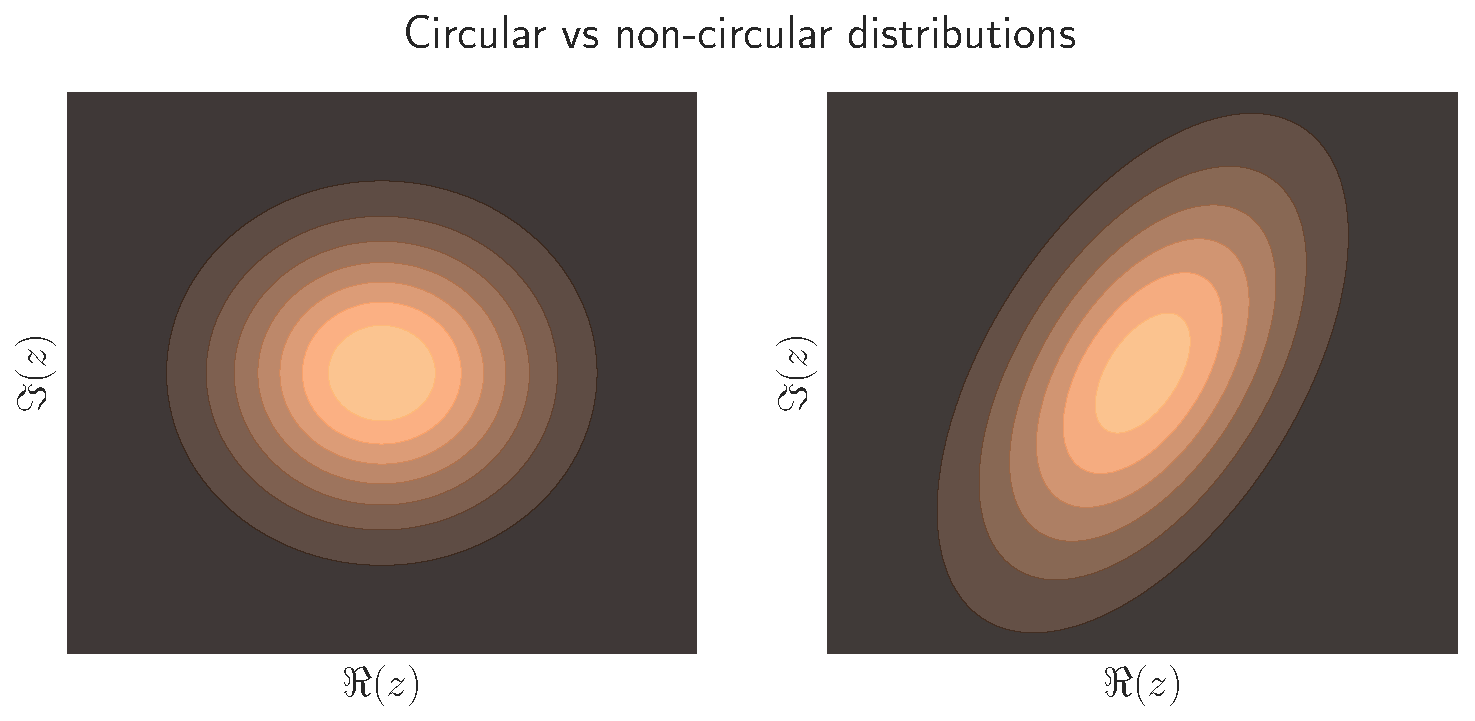
\includegraphics[scale=0.5]{pictures/std_cmplx_norm_distrib}
	\caption{Example of a perfectly circular distribution $(\rho_z=0)$ and a non-circular one (right).}
	\label{fig:circular_distrib}
\end{figure} 
In some papers, the circular quotient is defined as a covariance measure between $Z$ and $\bar{Z}$, so among a random variable and its complex conjugate, rather than considering real and imaginary parts. We believe that those formulations in the end are equivalent from a practical point of view, and so they can be used interchangeably.\\
From another perspective, a complex random vector $\vb{Z}$ is called circularly symmetric if, for every $\varphi\in[-\pi,\pi)$, the distribution of $e^{i\varphi}\vb{Z}$ is the same of $\vb{Z}$. The vector's PDF then satisfies $f(\vb{Z})=cg(\abs{\vb{Z}}^2)$ for some non-negative function $g$ and normalizing constant $c$. Hence, the regions of constant contours, for this distribution, are circles in the complex plane (as can be observed from figure \ref{fig:circular_distrib}).\\
Another interesting fact is that $\rho_Z$ possesses an intuitive geometrical interpretation since the modulus and phase of its principal square-root are equal to the eccentricity and angle of orientation of the ellipse defined by the covariance matrix of the real and imaginary parts of $Z$ \cite{circularity_geometric_interpretation}.


\section{Why not to prefer real-valued networks with two channels?}
As we explained in the previous section, complex numbers can also be represented as points in $\mathds{R}^2$, considering the "isomorphism" $\mathds{C}\ni x+iy \leftrightarrow (x,y)^T\in\mathds{R}^2$. Consequently, one of the main approaches that are followed when a complex input is fed to a real-valued model, is exactly to split such input into two independent channels, one for the real components and one for the imaginary. That's similar to what happens for the three channels of an RGB image, that are sent, one at a time independently, trough a convolutional (or fully-connected) layer.\\
Unfortunately, even tho this approach is efficient and coherent with the way complex numbers are managed in modern calculators (real and imaginary parts stored as separated floating point numbers), it turns out to be non-proper, even "dangerous", from an analytic point of view, since the real-valued inner product implemented in linear layers dismisses the mathematical correlation between the real and imaginary parts. 

 
\subsection*{Complex Multiplication}
\label{subsec:cmplx_multiplication}

\begin{figure}[!ht]
	\centering
	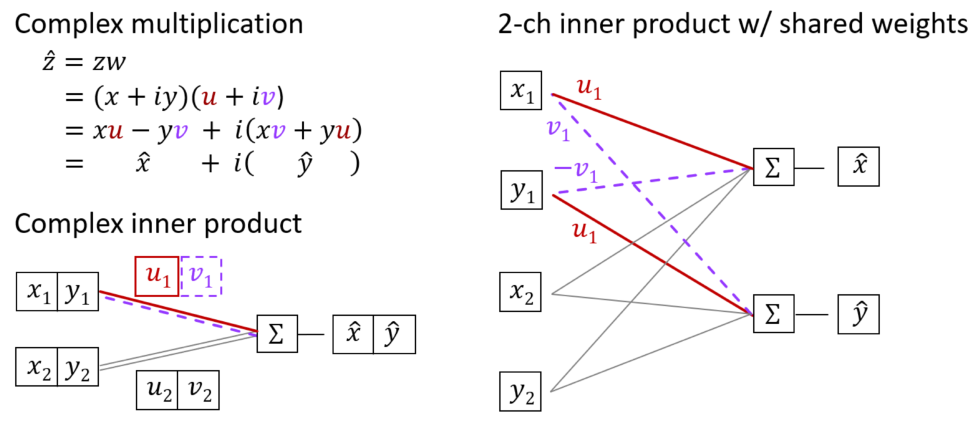
\includegraphics[width=\textwidth]{pictures/cmplx_multiplication.pdf}
	\caption{Visual representation of the multiplication and the corresponding implementation in a complex-valued network (bottom left). In order to replicate the same behavior on a real-valued network, the weights' components must be replicated, or shared, in the 2-channels layer (on the right) (source:\cite{Virtue:EECS-2019-126}).}
	\label{fig:cmplx_multiplication}
\end{figure}

Complex multiplication, in fact, has a specific protocol that combines the real and imaginary components of the input to the corresponding of the output (figure \ref{fig:cmplx_multiplication}, top left). In the case of a complex input that has been split into its components, trying to reproduce the multiplication using the naive real-valued implementation of the "inner product" breaks this protocol. The reason is simply that real and imaginary parts of the output depend on the constituents of both factors.\\
Nevertheless, it is possible to connect the (real-valued) network's components in order to "mimic" exactly the behavior of complex multiplication: you just need to exploit \textit{shared weights}, as in the example in figure \ref{fig:cmplx_multiplication} (on the right). However, this do not come without any cost, since $6x$ floating point operations are required (4 multiplications + 2 sums), with respect to a standard product, making this approach quite inefficient.\\
For a better understanding of the differences between complex and real multiplication it may be worth to give a look at figure \ref{fig:mult_dof}, in which are represented the various degrees of freedom of those operations. Complex multiplication naturally has two degrees of freedom, \textit{scaling} and \textit{rotation} (check \ref{obs:cmplx_mult_homothety}), compared to the four that characterize a product among vectors in $\mathds{R}^2$. Let's consider the black letter "R" in the image, as the input $z_{in}$ of a fully-connected layer in our network. This letter may change in different ways depending on the multiplication protocol implemented:
\begin{itemize}
	\item[-] with single-channel real weights (\ref{fig:mult_dof}, left), the only possible effects is a re-scaling of the input;
	\item[-] in the complex plane (\ref{fig:mult_dof}, center), as repeated several times, the multiplication depends on two parameters (magnitude and phase of the complex-valued weights) and represents and homothety in the plane;
	\item[-] if the multiplication is instead implemented with a real-valued layer with two inputs and two outputs (\ref{fig:mult_dof}, right), there are four weights to be learned; that will be for sure more expensive, but can guarantees two additional transformations like \textit{reflect} and \textit{shear} (bad or good thing depending on the dataset used).	
\end{itemize}

In many applications the relative change in phase between neighboring pixels may be of importance and the absolute phase value irrelevant. Two-channel real networks that treat real and imaginary parts independently can be problematic if a certain application needs to be invariant with respect to this arbitrary global complex scaling across an image. 

\begin{figure}[!ht]
	\centering
	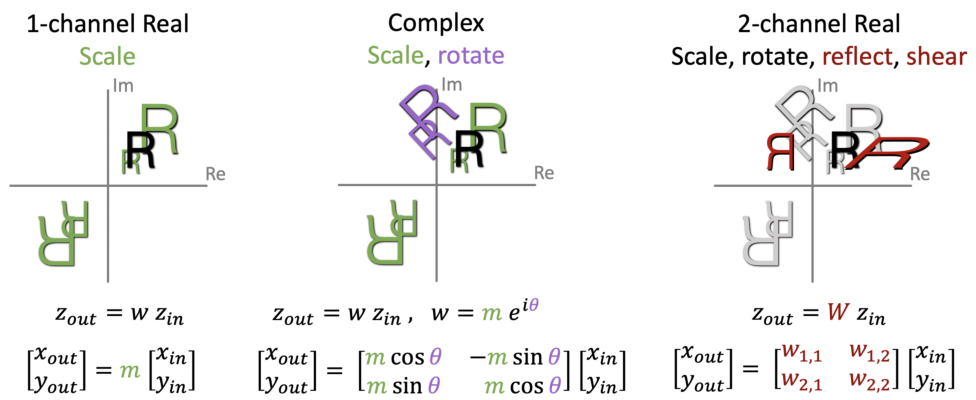
\includegraphics[width=\textwidth]{pictures/multiplication_dof.pdf}
	\caption{Visual representation of the complex multiplication (center) compared to its real-valued implementations (1-ch left, 2-ch right) (source:\cite{Virtue:EECS-2019-126}).}
	\label{fig:mult_dof}
\end{figure}


\subsection*{Non-Linear Activations}
Not only linear operations would be affected by this complex decomposition, but also non-linear ones. In generic neural networks, the main non-linear contribute is due to activation functions. But while complex multiplication can be in some way reproduced also by real-valued layers, for those non-linear activations the situation is not so straightforward. Working with a 2-channels input implies that the components will pass as independent variables trough the activation, which again dismisses eventual natural correlations between real and imaginary parts. Furthermore, when working, for example, with the canonical \texttt{ReLU} activation, one can fell into undesirable scenarios like a number with a large magnitude not allowed to pass (because of a negative component) or even unexpected rotations (because either real or imaginary parts got strongly altered). We cannot even renounce to them, since they are basically the core of a backpropagation algorithm. The only possibility, then, is to define a whole set of new activation functions, more suitable for working in $\mathds{C}$.\\
Later, we will see how the choice of the activation was one of the most discussed obstacles in developing a definitive complex-valued deep learning framework.


\end{document}
